\part{Celestial $\mathcal{A}$mplitudes \& CCFT}
% 计数器清零,每个part都要引用,除了part1
\setcounter{theorem}{0}
\setcounter{definition}{0}
\setcounter{lemma}{0}
\setcounter{sidenote}{1}
\section{Conformal basis}
QFT中利用费曼图计算散射振幅都是在动量空间下进行的,也就是选取在平面波为基底,这样做最大的好处是可以显现出平移对称性。但是在考虑天球上的散射问题时,很显然我们应当最大化利用共性对称性,所以基底应该选取为类似CFT中初级场的形式,称之为“Conformal Primary Wave Function”,这样$\mathbb{R}^{d+1,1}$上的散射振幅就有希望在这个基底下类似于CFT$_{d}$中的n点关联函数,Clifford Cheung很早就利用这个基底对一些特殊情形进行了研究\cite{Cheung:2016iub}。现在顺着文献\cite{Pasterski:2017kqt}的思路来介绍这一组基底。
\subsection{Massive Scalar}
\begin{definition}[Massive Scalar Conformal Primary Wave Function]
自旋为$0$的标量场既没有$\mathbb{R}^{d+1,1}$上的$SO(d+1,1\uparrow$指标,也没有spinning CFT特有的张量指标,或者说处于$SO(d)$的标量表示。对于平面波,我们使用在壳动量来标记基底,现在我们使用$\Delta\in\mathbb{C},\vec{w}$来标记基底。
\begin{itemize}
	\item 在壳:
	\begin{equation}
		\left(\frac{\partial}{\partial X^{\nu}} \frac{\partial}{\partial X_{\nu}}-m^{2}\right) \phi_{\Delta}\left(X^{\mu} ; \vec{w}\right)=0
	\end{equation}
	\item 在共形变换和$SO(d+1,1)$下协变:
	\begin{equation}
		\phi_{\Delta}\left({\Lambda^{\mu}}_{\nu} X^{\nu} ; \vec{w}^{\prime}(\vec{w})\right)=\left|\frac{\partial \vec{w}^{\prime}}{\partial \vec{w}}\right|^{-\Delta / d} \phi_{\Delta}\left(X^{\mu} ; \vec{w}\right)
	\end{equation}
	这里$\vec{w}\to\vec{w}^\prime$是共形变换\footnote{注意,对于$d=2$的情形,对应的是全局共形变换,更类似于准初级场。},${\Lambda^\mu}_\nu$是诱导的Lorentz变换。
\end{itemize}
\end{definition}
后面的讨论使用Embedding形式将$\mathbb{R}^{d}$嵌入到$\mathbb{R}^{d+1,1}$的光锥,再次写下这个嵌入:
\begin{equation}
	q^\mu(\vec{w})=\left(1+|\vec{w}|^2,2\vec{w},1-|\vec{w}|^2\right),\quad q^\mu(\vec{w}^\prime)=\left|\frac{\partial \vec{w}^\prime}{\partial\vec{w}}\right|^{\frac{1}{d}}{\Lambda^\mu}_\nu q^\nu(\vec{w})
\end{equation}
粒子在壳动量$p^2=-m^2$,由于质量是固定的,抽出动量方向得到$\hat p^2=-1$,而这其实就说明$\hat p$位于unit hyperboloid space $\mathbb{H}_{d+1}$上\sn{$\mathbb{H}_{d+1}$表示$d+1$维截面曲率恒为$-1$的超曲面,Killing-Hopf定理保证这样的曲面只有这一种}。可以利用Poincar\'e half-plane对$\mathbb{H}_{d+1}$进行参数化:
\begin{equation}
	ds^2_{\mathbb{H}_{d+1}}=\frac{dy^2+d\vec{z}\cdot d\vec{z}}{y^2},\quad y>0,\vec{z}\in\mathbb{R}^d
\end{equation}
$y=0$对应$\partial\mathbb{H}_{d+1}$。$ds^2_{\mathbb{H}_{d+1}}$天然是$SO(d+1,1)$不变的,也就是在下面的变换下不变:
\begin{itemize}
	\item $\mathbb{R}^d$ translation : $\quad y^{\prime}=y, \quad \vec{z}^{\prime}=\vec{z}+\vec{a}$,\\
	\item $S O(d)$ rotation : $y^{\prime}=y, \quad \vec{z}^{\prime}=M \cdot \vec{z}$,\\
	\item dilation : $\quad y^{\prime}=\lambda y, \quad \vec{z}^{\prime}=\lambda \vec{z}$\\
	\item special conformal transformation : $y^{\prime}=\frac{y}{1+2 \vec{b} \cdot \vec{z}+|\vec{b}|^2\left(y^2+|\vec{z}|^2\right)}, \quad \vec{z}^{\prime}=\frac{\vec{z}+\left(y^2+|\vec{z}|^2\right) \vec{b}}{1+2 \vec{b} \cdot \vec{z}+|\vec{b}|^2\left(y^2+|\vec{z}|^2\right)}$
\end{itemize}
任意在在壳动量$m\hat p$可以参数化为:
\begin{equation}
	\hat{p}(y,\vec{z})=\left(\frac{1+y^2+|\vec{z}|^2}{2y},\frac{\vec{z}}{y},\frac{1-y^2-|\vec{z}|^2}{2y}\right)
\end{equation}
这其实就是在将$\mathbb{H}_{d+1}$嵌入到$\mathbb{R}^{d+1,1}$的未来光锥部分\sn{因为$\hat p^0>0$},比如$\mathbb{R}^{3,1}$的时空图就可以分层为:
\begin{figure}[H]
	\centering 
	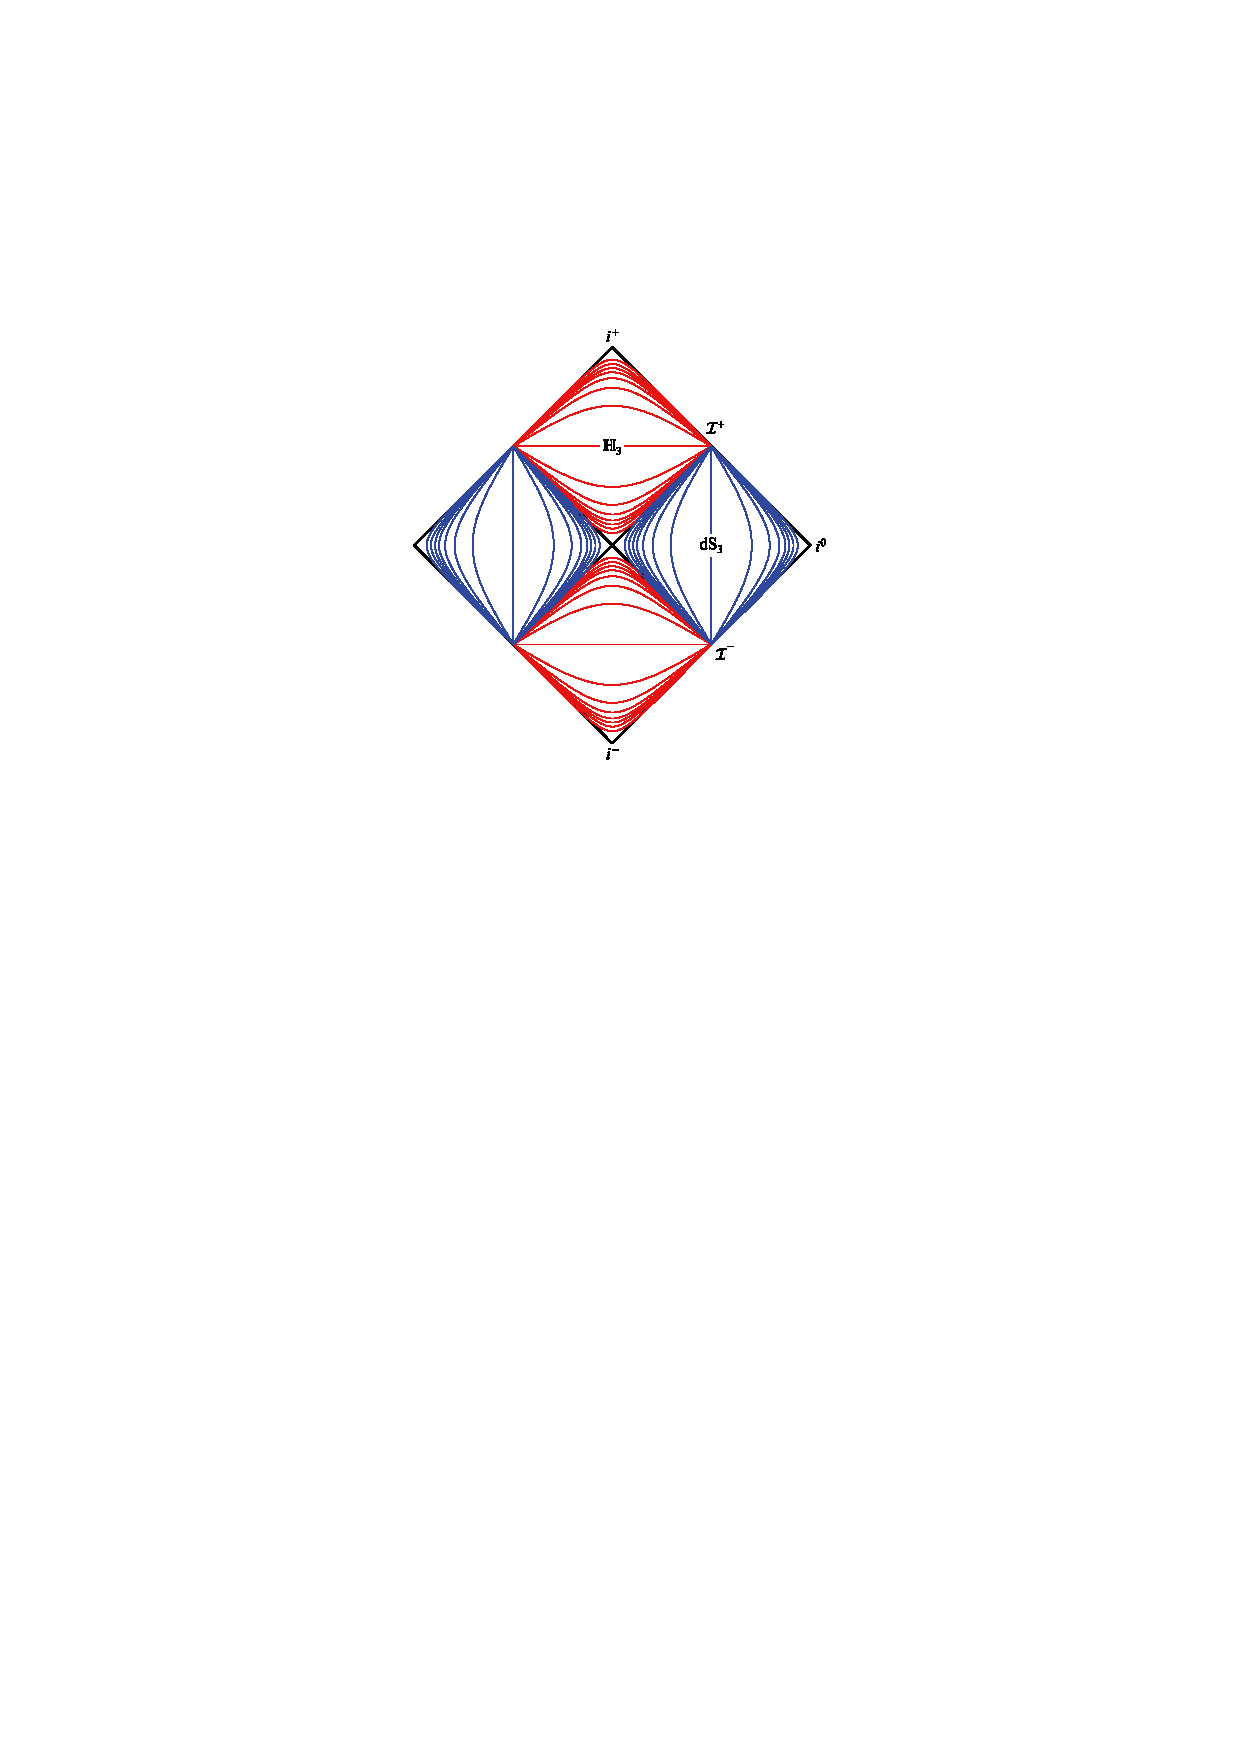
\includegraphics{figs/fig6.pdf}
	\caption{$Mink_4$时空的叶状结构}
\end{figure}
我们只使用unit的那一层。AdS/CFT对偶里面有一个bulk-to-boundary传播子,在前面的参数化下定义为\cite{Witten:1998qj}:
\begin{equation}
	\boxed{
	G_\Delta(\hat{p};\vec{w})=\left(\frac{y}{y^2+|\vec{z}-\vec{w}|^2}\right)^\Delta =G_\Delta(\hat{p};q)=\frac{1}{(-\hat{p}\cdot q)^\Delta}
	}
\end{equation}
这个传播子在共形变换$q\to q^\prime$,以及所诱导的Lorentz变换$\hat p\to\hat p^\prime$下变换性质为:
\begin{equation}
	G_\Delta(\hat{p'};q')=\left|\frac{\partial\vec{w}'}{\partial\vec{w}}\right|^{-\Delta/d}G_\Delta(\hat{p};q)
\end{equation}
最终的基底肯定是用平面波$\exp\left[\pm im\hat{p}\cdot X\right]$线性组合得到的,这里$+$表示out态,$-$表示in态。而且线性组合要对所有在壳动量构成的平面波求和,所以积分是在$\mathbb{H}_{d+1}$上进行的,积分测度是上面的不变测度:
\begin{equation}
	\int_{\mathbb{H}_{d+1}}[d\hat{p}]\equiv\int_0^\infty\frac{dy}{y^{d+1}}\int d^d\vec{z}=\int_{\hat p^2=-1}\frac{d^{d+1}\hat{p}^i}{\hat{p}^0}
\end{equation}
由于KG方程是一个线性方程,所以线性组合之后的结果都是KG方程的解\sn{只要线性组合的系数与$X$无关就好}。由于$G_\Delta$在共形变换下刚好出来我们需要的共形变换因子,而诱导的Lorentz变换本身不贵改变$\hat p \cdot X$和积分测度,所以下面的积分就是满足条件的conformal basis:
\begin{equation}\label{27}
	\boxed{
	\phi_\Delta^\pm(X^\mu;\vec{w})=\int_{\mathbb{H}_{d+1}}[d\hat{p}]G_\Delta(\hat{p};\vec{w})\exp\left[\pm im\hat{p}\cdot X\right]
	}
\end{equation}
注意$\Delta$和$\vec{w}$是用来标记基底的,与$m$无关。但是上面的式子只是形式上的定义,第一不便于计算,第二上式对于$m\in\mathbb{R}_+$是发散的,只有对于$m\in-i{\mathbb{R}_+}$才收敛,所以上式应当看作是先把$m$变成纯虚数积分,然后延拓到实轴。所以考虑直接去找满足条件的KG方程的解,设试探解为:
\begin{equation}
	\phi_\Delta(X^\mu;\vec{w})=\frac{f(X^2)}{(-q\cdot X)^\Delta}
\end{equation}
代入方程得到:
\begin{equation}
	0=4X^2f''(X^2)-2(2\Delta-d-2)f'(X^2)-m^2f(X^2)
\end{equation}
这是虚宗量Bessel方程,考虑$X\to\infty$收敛的解,解正比于第二类修正Bessel函数:
\[f(X^2)\propto\left(\sqrt{-X^2}\right)^{\Delta-\frac{d}{2}}K_{\Delta-\frac{d}{2}}\left(m\sqrt{X^2}\right)\]
前面的比例系数可以从积分表达式\ref{27}积分后最终对比得到:
\begin{equation}
	\phi_\Delta^\pm(X^\mu;\vec{w})=\frac{2^{\frac d2+1}\pi^{\frac d2}}{(im)^{\frac d2}}\frac{(\sqrt{-X^2})^{\Delta-\frac d2}}{(-q(\vec{w})\cdot X\mp i\epsilon)^\Delta}K_{\Delta-\frac d2}(m\sqrt{X^2})
\end{equation}
$\mathcal{A}\equiv\bra{\textbf{out}}\mathcal{S}\ket{\text{in}}$,那么在conformal基底下的散射振幅和原先动量空间散射振幅之间关系为:
\begin{equation}
	\widetilde{\mathcal{A}}(\Delta_i,\vec{w}_i)\equiv\prod_{k=1}^n\int_{\mathbb{H}_{d+1}}[d\hat{p}_k]G_{\Delta_k}(\hat{p}_k;\vec{w}_k)\mathcal{A}(\pm m_i\hat{p}_i^\mu)
\end{equation}
显然其具有CFT中n点关联函数性质:
\begin{equation}
	\widetilde{\mathcal A}(\Delta_{i},\vec{w}_{i}^{\prime}(\vec{w}_{i}))=\prod_{k=1}^{n}\left|\frac{\partial\vec{w}_{k}^{\prime}}{\partial\vec{w}_{k}}\right|^{-\Delta_{k}/d}\widetilde{\mathcal A}(\Delta_{i},\vec{w}_{i})
\end{equation}

前面一直在讲基底,但前面不对$\Delta$进行限制,构造出来的$\{\phi^{\pm}_{\Delta,\vec{w}}\}$极有可能是超完备的。下面我们要干的事情是在构造出来的这些基底里面选某一簇构造正交完备归一基底。

\begin{definition}[shadow transformation]
	对于一个共形维数为$\Delta$的(准)初级场$\mathcal{O}_\Delta(\vec{w})$,其\textbf{shadow}的定义为\cite{Ferrara:1972xe,Ferrara:1972ay,Ferrara:1972uq,Ferrara:1972kab}:
	\begin{equation}
		\begin{aligned}\widetilde{\mathcal{O}}_\Delta(\vec{w})&\equiv\frac{\Gamma(\Delta)}{\pi^{\frac{d}{2}}\Gamma(\Delta-\frac{d}{2})}\int d^d\vec{w}'\frac{1}{|\vec{w}-\vec{w}'|^{2(d-\Delta)}}\mathcal{O}_\Delta(\vec{w}')\end{aligned}
	\end{equation}
	不难发现,场的shadow变成了共形维数为$d-\Delta$的(准)初级场。
\end{definition}
由于$K_\alpha=K_{-\alpha}$,以及下面的恒等式\cite{Simmons-Duffin:2012juh}:
\begin{equation}
	\int d^{d}\vec{z}\frac{1}{|\vec{z}-\vec{w}|^{2(d-\Delta)}}\frac{1}{(-q(\vec{z})\cdot X)^{\Delta}}=\frac{\pi^{\frac{d}{2}}\Gamma(\Delta-\frac{d}{2})}{\Gamma(\Delta)}\frac{(-X^{2})^{\frac{d}{2}-\Delta}}{(-q(\vec{w})\cdot X)^{d-\Delta}}
\end{equation}
得到了一个核心等式:
\begin{equation}\label{eq:27.17}
	\boxed{\widetilde{\phi_\Delta^\pm}(X;\vec{w})=\phi_{d-\Delta}^\pm(X;\vec{w})}
\end{equation}
这实际上直接把空间一分为二,分成某个子空间和它的shadow,我们只用取其中一个构成基就好,因为它的shadow是其线性组合。

在考虑$SO(d+1,1)$的无限维表示\sn{\cite{Sun:2021rrs,Sun:2021thf}这两篇文章比较易读,而且重在比较新,文章\cite{Bissi:2023bhv}的$\S 2.2$是对此内容的一个简短review,更多的阅读材料可以在那里找到。}时会出现所谓\textbf{principal continuous series}的概念:
\begin{equation}
	\boxed{\Delta\in\frac d2+i\mathbb{R}}
\end{equation}
后面构造conformal basis就是用这一series里面的$\Delta$或其子集进行构造,这一点不加证明,后面只是去说明这样确实能得到正确的基底。

首先注意到关于$G_\Delta$的几个正交完备性关系\cite{Costa:2014kfa}:
\begin{equation}
	\int_{-\infty}^{\infty}d\nu\mu(\nu)\int d^{d}\vec{w}G_{\frac{d}{2}+i\nu}(\hat{p}_{1};\vec{w})G_{\frac{d}{2}-i\nu}(\hat{p}_{2};\vec{w})=\delta^{(d+1)}(\hat{p}_{1},\hat{p}_{2})
\end{equation}
这里$\delta$函数是定义在$\mathbb{H}_{d+1}$上也就是$SO(d+1,1)$不变的,积分测度$\mu(\nu)$:
\begin{equation}
	\mu(\nu)=\frac{\Gamma(\frac d2+i\nu)\Gamma(\frac d2-i\nu)}{4\pi^{d+1}\Gamma(i\nu)\Gamma(-i\nu)}
\end{equation}
还有一个
\begin{equation}
	\begin{gathered}
		\int_{H_{d+1}}[d\hat{p}]G_{\frac d2+i\nu}(\hat{p};\vec{w}_{1})G_{\frac d2+i\bar{\nu}}(\hat{p};\vec{w}_{2})= \\
		2\pi^{d+1}\frac{\Gamma(i\nu)\Gamma(-i\nu)}{\Gamma(\frac d2+i\nu)\Gamma(\frac d2-i\nu)}\delta(\nu+\bar{\nu})\delta^{(d)}(\vec{w}_{1}-\vec{w}_{2})+2\pi^{\frac d2+1}\frac{\Gamma(i\nu)}{\Gamma(\frac d2+i\nu)}\delta(\nu-\bar{\nu})\frac{1}{|\vec{w}_{1}-\vec{w}_{2}|^{2(\frac d2+i\nu)}}.
	\end{gathered}
\end{equation}
利用这些关系可以得到\ref{27}的逆变换:
\begin{equation}
	\boxed{e^{\pm im\hat{p}\cdot X}=2\int_0^\infty d\nu\mu(\nu)\int d^d\vec{w}G_{\frac d2-i\nu}(\hat{p};\vec{w})\phi_{\frac d2+i\nu}^\pm(X^\mu;\vec{w})}
\end{equation}
由于平面波基底完备,逆变换的存在性立刻就说明了利用principal continuous series构造出来的$\{\phi^{\pm}_{\Delta,\vec{w}}\}$也完备,而且注意到我们这里利用\ref{eq:27.17}将$\nu$限制在了$\mathbb{R}_+$上,所以:
\begin{equation}\label{eq:27.23}
	\boxed{\Delta\in\frac d2+i\mathbb{R}_{\geq 0}}
\end{equation}
这佐证了前面提到的只需要在空间和其shadow里面取一个就好了。正交性依赖于内积的定义,这里自然的定义KG内积:
\begin{equation}
	(\Phi_1,\Phi_2)=-i\int_\Sigma d^{d+1}X^i\left[\Phi_1(X)\partial_{X^0}\Phi_2^*(X)-\partial_{X^0}\Phi_1(X)\Phi_2^*(X)\right]
\end{equation}
这个定义是Poincar\'e不变的,是与Cauchy面选取无关的。计算得到:
\begin{equation}
	\begin{aligned}
		\left(\phi_{\frac{d}{2}+i\nu_{1}}^{\pm}(X^{\mu};\vec{w_{1}})\right.,&\left.\phi_{\frac{d}{2}+i\nu_{2}}^{\pm}(X^{\mu};\vec{w_{2}})\right) \\
		=&\pm\frac{2^{d+3}\pi^{2d+2}}{m^{d}}\frac{\Gamma(i\nu_{1})\Gamma(-i\nu_{1})}{\Gamma(\frac{d}{2}+i\nu_{1})\Gamma(\frac{d}{2}-i\nu_{1})}\delta(\nu_{1}-\nu_{2})\delta^{(d)}(\vec{w}_{1}-\vec{w}_{2}) \\
		&\pm\cancelto{0}{\frac{2^{d+3}\pi^{\frac{3d}{2}+2}}{m^{d}}\frac{\Gamma(i\nu_{1})}{\Gamma(\frac{d}{2}+i\nu_{1})}\delta(\nu_{1}+\nu_{2})\frac{1}{|\vec{w}_{1}-\vec{w}_{2}|^{2(\frac{d}{2}+i\nu_{1})}}}
	\end{aligned}
\end{equation}
第二项为$0$是因为\ref{eq:27.23}。总结一下,我们得到了$\ket{\text{in}}$和$\ket{\text{out}}$态的基底为:
\begin{equation}
	\boxed{\mathcal{B}^{\pm}=\left\{\begin{array}{c|c}\phi_{\frac{d}{2}+i\nu}^{\pm}(X;\vec{w})&\nu\geq0,\vec{w}\in\mathbb{R}^d\end{array}\right\}}
\end{equation}
它的shadow同样是一组基底:
\begin{equation}
	\boxed{\widetilde{\mathcal{B}}^\pm=\left\{\begin{array}{c|c}\phi_{\frac{d}{2}+i\nu}^\pm(X;\vec{w})&\nu\le0,\vec{w}\in\mathbb{R}^d\end{array}\right\}}
\end{equation}
\subsection{Massless Scalar}
无质量情况看作是有质量情况的极限,作换元$\omega\equiv\frac{m}{2y}$,积分核有如下渐近行为:
\begin{equation}
	G_{\Delta}(y,\vec{z};\vec{w})\xrightarrow{m\to0}\pi^{\frac{d}{2}}\frac{\Gamma(\Delta-\frac{d}{2})}{\Gamma(\Delta)}y^{d-\Delta}\delta^{(d)}(\vec{z}-\vec{w})+\frac{y^{\Delta}}{|\vec{z}-\vec{w}|^{2\Delta}}+\cdots 
\end{equation}
计算得到:
\begin{equation}
	\begin{aligned}\phi_{\frac{d}{2}+i\nu}^{\pm}(X;\vec{w})\xrightarrow{m\to0}&\left(\frac{m}{2}\right)^{-\frac{d}{2}-i\nu}\frac{\pi^{\frac{d}{2}}\Gamma(i\nu)}{\Gamma(\frac{d}{2}+i\nu)}\int_{0}^{\infty}d\omega\omega^{\frac{d}{2}+i\nu-1}e^{\pm i\omega q(\vec{w})\cdot X}\\+&\left(\frac{m}{2}\right)^{-\frac{d}{2}+i\nu}\int d^{d}\vec{z}\frac{1}{|\vec{z}-\vec{w}|^{2(\frac{d}{2}+i\nu)}}\int_{0}^{\infty}d\omega\omega^{\frac{d}{2}-i\nu-1}e^{\pm i\omega q(\vec{z})\cdot X}\end{aligned}
\end{equation}
上面的极限不是well-define的,因为$m^{\pm i\nu}$,但这是个相位,不妨先丢掉,而第二项是第一项的shadow,所以猜测最终应该是下面的形式:
\begin{equation}
	\boxed{\varphi_\Delta^\pm(X^\mu;\vec w)\equiv\int_0^\infty d\omega\omega^{\Delta-1}e^{\pm i\omega q\cdot X-\epsilon\omega}=\frac{(\mp i)^\Delta\Gamma(\Delta)}{(-q(\vec w)\cdot X\mp i\epsilon)^\Delta}}
\end{equation}
其中$\Delta\in\mathbb{C}$,需要重新去找寻。这个式子的形式就是所谓\textbf{Mellin变换},可以解释成对未来光锥上的某一条射线积分,也就是把所有同“方向”,不同“能量”的平面波组合。上面变换的逆变换为:
\begin{equation}
	e^{\pm i\omega q\cdot X-\epsilon\omega}=\int_{-\infty}^{\infty}\frac{d\nu}{2\pi}\omega^{-\Delta}\frac{(\mp i)^{\Delta}\Gamma(
		\Delta)}{(-q\cdot X\mp i\epsilon)^{\Delta}},\quad\omega>0,\Re(\Delta)>0
\end{equation}
这说明了$\Re(\Delta)>0$就能保证完备性,而且这组基底张成的空间中很重要的一点是不含零动量的平面波解\sn{这一点是必须的,因为他是KG方程没有物理意义的解,要抛弃掉}。如果选取$\Re(\Delta)=\frac{d}{2}$,$\Im(\Delta)\in\mathbb{R}$,则:
\begin{equation}
	\begin{pmatrix}\varphi_{\frac{d}{2}+i\nu_{1}}^{\pm}(X^{\mu};\vec{w}_{1}),\varphi_{\frac{d}{2}+i\nu_{2}}^{\pm}(X^{\mu};\vec{w}_{2})\end{pmatrix}=\pm8\pi^{d+2}\delta(\nu_{1}-\nu_{2})\delta^{(d)}(\vec{w}_{1}-\vec{w}_{2})
\end{equation}
这个时候注意shadow:
\begin{equation}
	\begin{aligned}
		\widetilde{\varphi_{\frac{d}{2}+i\nu}^{\pm}}(X^{\mu};\vec{w})& =\frac{\Gamma(\frac{d}{2}+i\nu)}{\pi^{\frac{d}{2}}\Gamma(i\nu)}\int d^{d}\vec{z}\frac{1}{|\vec{z}-\vec{w}|^{2(\frac{d}{2}-i\nu)}}\varphi_{\frac{d}{2}+i\nu}^{\pm}(X^{\mu};\vec{z})  \\
		&=(\mp i)^{\frac d2+i\nu}\Gamma(\frac d2+i\nu)\frac{(-X^2)^{-i\nu}}{(-q(\vec{w})\cdot X\mp i\epsilon)^{\frac d2-i\nu}}\\
		\left(\varphi_{\frac{d}{2}+i\nu_1}^{\pm}(X^{\mu};\vec{w_1}),\right.&\left.\widetilde{\varphi_{\frac{d}{2}+i\nu_2}^{\pm}}(X^{\mu};\vec{w_2})\right)=\pm8\pi^{\frac{d}{2}+2}\frac{\Gamma(\frac{d}{2}-i\nu_1)}{\Gamma(-i\nu_1)}\delta(\nu_1-\nu_2)\frac{1}{|\vec{w_1}-\vec{w_2}|^{2(\frac{d}{2}+i\nu_1)}}
	\end{aligned}
\end{equation}
其shadow当然也是一组基底,但并不是$\nu\to-\nu$这么简单了,这导致$\nu$的取值范围也拓宽到了所有实数。总结一下,我们得到了Massless scalar的conformal basis:
\begin{equation}
	\boxed{\mathcal{B}_{m=0}^{\pm}=\left\{\begin{array}{c|c}\varphi_{\frac{d}{2}+i\nu}^{\pm}(X^{\mu};\vec{w})&\nu\in\mathbb{R},\vec{w}\in\mathbb{R}^{d}\end{array}\right\}}
\end{equation}
其shadow也可以作为一组基:
\begin{equation}
	\boxed{\widetilde{\mathcal{B}}_{m=0}^{\pm}=\left\{\begin{array}{c|c}\widetilde{\varphi_{\frac{d}{2}+i\nu}^{\pm}}(X^{\mu};\vec{w})&\nu\in\mathbb{R},\vec{w}\in\mathbb{R}^{d}\end{array}\right\}}
\end{equation}
\subsection{Phonton \& Graviton}
这两个除了自旋不为0,还有一个比较麻烦的点是需要取定规范。
\subsection{Fermions}
\subsection{Restrict to Mink$_{4}$}
\subsection{Example: 2 massless and 1 massive scalars at tree\mbox{–}level}